\documentclass[12pt, a4paper]{article}

\usepackage[english]{babel}
\usepackage{lmodern}
\usepackage[utf8]{inputenc}
\usepackage[T1]{fontenc}
\usepackage[pdftex]{graphicx}
\usepackage{amsmath, amssymb}
\usepackage[hidelinks,unicode]{hyperref}
\usepackage{float}
\usepackage{listings}
\usepackage{tikz}
\usepackage{xcolor}
\usepackage{tabularx}
\usepackage[final]{pdfpages}
\usepackage{syntax}
\usepackage{caption}
\usepackage{subcaption}
\usepackage{amsfonts}
\usepackage{wrapfig}
\usepackage{listingsutf8}

\definecolor{mauve}{rgb}{0.58,0,0.82}
\usetikzlibrary{shapes,positioning,matrix,arrows}

\newcommand{\img}[1]{(see figure \ref{#1})}
\newcommand\todo[1]{\textcolor{red}{#1}}

\definecolor{pblue}{rgb}{0.13,0.13,1}
\definecolor{pgreen}{rgb}{0,0.5,0}
\definecolor{pred}{rgb}{0.9,0,0}
\definecolor{pgrey}{rgb}{0.46,0.45,0.48}


\lstdefinestyle{flex}{
    frame=tb,
    aboveskip=3mm,
    belowskip=3mm,
    showstringspaces=false,
    columns=flexible,
    basicstyle={\small\ttfamily},
    numbers=none,
    numberstyle=\tiny\color{black},
    keywordstyle=\color{black},
    commentstyle=\color{black},
    stringstyle=\color{black},
    breaklines=true,
    breakatwhitespace=true,
    tabsize=3
}

%define Javascript language
\lstdefinelanguage{JavaScript}{
    keywords={const, typeof, new, true, false, catch, function, return, null, catch, switch, var, if, in, while, do, else, case, break},
    keywordstyle=\color{blue}\bfseries,
    ndkeywords={default, class, export, boolean, throw, implements, import, this},
    ndkeywordstyle=\color{darkgray}\bfseries,
    identifierstyle=\color{black},
    sensitive=false,
    comment=[l]{//},
    morecomment=[s]{/*}{*/},
    commentstyle=\color{pgreen}\ttfamily,
    stringstyle=\color{mauve}\ttfamily,
    morestring=[b]',
    morestring=[b]"
}

\lstset{
    frame=tb,
    language=Python,
    aboveskip=3mm,
    belowskip=3mm,
    showstringspaces=false,
    columns=flexible,
    basicstyle={\small\ttfamily},
    numbers=none,
    numberstyle=\tiny\color{gray},
    keywordstyle=\color{blue},
    commentstyle=\color{pgreen},
    stringstyle=\color{mauve},
    breaklines=true,
    breakatwhitespace=true,
    tabsize=3,
     literate=%
         {á}{{\'a}}1
         {í}{{\'i}}1
         {é}{{\'e}}1
         {ý}{{\'y}}1
         {ú}{{\'u}}1
         {ó}{{\'o}}1
         {ě}{{\v{e}}}1
         {š}{{\v{s}}}1
         {č}{{\v{c}}}1
         {ř}{{\v{r}}}1
         {ž}{{\v{z}}}1
         {ď}{{\v{d}}}1
         {ť}{{\v{t}}}1
         {ň}{{\v{n}}}1                
         {ů}{{\r{u}}}1
         {Á}{{\'A}}1
         {Í}{{\'I}}1
         {É}{{\'E}}1
         {Ý}{{\'Y}}1
         {Ú}{{\'U}}1
         {Ó}{{\'O}}1
         {Ě}{{\v{E}}}1
         {Š}{{\v{S}}}1
         {Č}{{\v{C}}}1
         {Ř}{{\v{R}}}1
         {Ž}{{\v{Z}}}1
         {Ď}{{\v{D}}}1
         {Ť}{{\v{T}}}1
         {Ň}{{\v{N}}}1                
         {Ů}{{\r{U}}}1    
}


\let\oldsection\section
\renewcommand\section{\clearpage\oldsection}

\begin{document}
	% this has to be placed here, after document has been created
	% \counterwithout{lstlisting}{chapter}
	\renewcommand{\lstlistingname}{Source code example}
	\renewcommand{\lstlistlistingname}{List of code example}
    \begin{titlepage}

        \centering

        \vspace*{\baselineskip}
        \begin{figure}[H]
        \centering
        
\includegraphics[width=7cm]{img/fav-logo.jpg}
        \end{figure}

        \vspace*{1\baselineskip}

        \vspace{0.75\baselineskip}

        \vspace{0.5\baselineskip}
        {KIV/VSS Semester Project}

        {\LARGE\sc Benchmarking A Payment Terminal Managemenent Server \\}

        \vspace{4\baselineskip}

        \vspace{0.5\baselineskip}

        {\sc\Large Stanislav Král \\}
        \vspace{0.5\baselineskip}
        {A20N0091P}

        \vfill

        {\sc Západočeská univerzita v Plzni\\
        Fakulta aplikovaných věd}

    \end{titlepage}

    % TOC
    \tableofcontents
    \pagebreak

\section{Tools for benchmarking web applications}\label{intro}

With the number of people with access to the Internet continuously rising the usage load of web applications is obviously rising too and the need for scalable web technologies and architectures is higher than ever.
While today's web developers are aware of this they are also in need of tools that are able to measure application's performance and to discover its possible limits.

Many free and paid tools for benchmarking web applications are available today.
One example of such free tool is Apache's open-source program \textbf{ab} (also known as ApacheBench) that has been available since 1996 and was originally used to test the Apache HTTP Server.
However, it's generic enough to test any web server supporting HTTP protocols.
One of its main disadvantages is the fact that it allows tests to be run only in one thread which limits concurrency and may create bottlenecks.
This problem can be overcome by running multiple instances of the program.

Shortly after the release of ApacheBench Apache releases another tool for benchmarking web applications -- \textbf{Apache JMeter}.
Unlike its predecessor Apache JMeter comes with a rich GUI and feature set and is capable of measuring the performance not only of HTTP servers but also of other services such as JDBC database connections, FTP, LDAP or JMS.
Out of the box it supports test parametrization, response validation, per-thread cookies, integration with the Selenium test framework and variety of useful reports.
JMeter architecture is focused around plugins and missing features not present in the base version of the program are added via official or community plugins.

With the promise of making the process of defining and writing load tests simpler and more intiutive for developers the open-source load testing tool \textbf{k6} is released in 2016.
It is used for testing the performance and realiability of web APIs, microservices and websites.
When using this tool developers use the Javascript language to write benchmark scenarios, where each simulated user (that makes request to the application put under a test) is represented by a Virtual User entity and its behaviour can be defined in a single Javascript method.
The number of users can be easily defined in such way that it will be changing during the test as needed by the test scenario (e.g., linear growth in the first 60 seconds followed by a constant number of users).
Once the test is finished the user is presented with a brief summary containing useful stats such as the average duration of each stage of performed HTTP requests.
In addition to the tool the team behind it offers a paid online service that allows for running load tests from the cloud with the possibility of creating advanced reports an summaries.
Even though running the tool locally is sufficient for most of the time and enough stress can be put on the tested server the reports of tests are missing some important information such as a chart with the average server response time during the test.
Luckily the tool makes it possible to serialize all events that occur during the test to a JSON file.
Such file can be then processed by our own software for visualization. 


\section{Automatization of terminal management}

As introduced in the assignment of this semester project the web application to be put under the test is the Dotypay Portal site that is used for the management of Dotypay payment terminals.

For the purpose of running benchmarks the Dotypay Portal development team has prepared a dedicated application instance running on the same configuration as the production instance.
However, the application's data in the instance to be tested were copied from the development environment.
This means that it was required to generate and submit additional data to the instance as it was excepted that the number of terminals present in the database (about 250 terminals)  would not be enough for putting enough stress on the server.

Because the server does not expose a REST API for creating new terminals the only way of filling the database with more data was to login into the application, go to the page where the form for creating new terminals is located and fill in individual terminal data. 
The initial goal was to have at least two thousand terminals present in the database.
Adding this many terminals manually would be close to unfeasable and a need for task automatization emerged.


\subsection{Writing an automatization script in Python}

Since the author of this semester project had previous experience with testing web applications using the Python language and the Playwright library\footnote{\url{https://playwright.dev/}} he chose write an automatization script using them.

It was soon discovered that not only the creation of terminals was required, but so was their activation, since only after terminals are activated they can communicate with the server using a unique API key that is assigned to them.

After a quick analysis of the application's UI interface and it's REST API (documented using OpenAPI specification) a Python script was created, that automates the process of logging in and creating a desired number of terminals.
Another feature of the script is that all terminals specified by a range of identifiers are activated.
The process of activation may include deactivation that is done using the UI interface and a REST API call that, if successful, yields an API key.


\subsection{Gathering terminal data}

Before running any benchmarks it was not only required to have a set of all terminal API keys of terminals present in the database but also to have other terminal data, such as their ID or serial number because it was required by some API calls present in test scenarios.
Even though this data could be accessed from the application's UI it would require another automatization script.
Because of that the author of this semester project was granted an access and login credentials to the instance's MS SQL database from which, using a simple SQL query, he was able to fetch all required data when needed.


\section{Benchmark scenarios}

In order to be able to measure application's ability to handle a higher amount of terminals it was required to prepare one or more benchmark scenarios that attempt to simulate real terminal behaviour.


\subsection{Terminal synchronization}

All terminals periodically perform a synchronization with the Dotypay portal.
This behaviour was described in the assignment but after further analysis of the Dotypay Payment Terminal application's source code it was soon discovered that the original description was quite shallow and the whole process of terminal synchronization involves more steps.
Synchronization consists of calling Dotypay Portal API endpoints in the following order:

\begin{itemize}
    \item \texttt{files} endpoint -- an endpoint that returns all files that the terminal should download (may involve any important documents or other files),
    \item \texttt{status} endpoint -- an endpoint that is used to report the status of the terminal to the server,
    \item \texttt{tasks} endpoint -- an endpoint that returns tasks (apply new terminal configuration or upload required files) filtered by their status (\texttt{CREATED}, \texttt{RECEIVED}, \texttt{IN\_PROGRESS}),
    \item and \texttt{apps} endpoint -- an endpoint that returns links to all APK files (Android application package file) to be downloaded and installed by the terminal filtered by their type (Launcher Application package, mandatory applications or optional applications).
\end{itemize}

Once terminal performs a synchronization it waits for a random duration of time ranging from 9 to 11 minutes before performing another synchronization.

The aim is to simulate at least 10 000 terminals periodically performing synchronization for the duration of 1 hour.

\subsection{Submission of performed transactions}

Every transaction that is performed by a terminal is submitted to the Dotypay portal so that it can be later used for sales analysis.
Transactions are submitted by calling the \texttt{transactions} endpoint with the transaction data in the request body.

The \texttt{transactions} endpoint allows for submitting one or more transactions, however, terminals usually submit only one transaction per request since they do so right after a transaction is performed.
Batch submission is done only when a previous transaction submission has failed and the terminal has already performed another transaction.
In that that case multiple transactions are sent in one request.

\begin{lstlisting}[language=JavaScript, caption={Transaction submission request body},captionpos=b, basicstyle=\tiny]
{
  "transactions": [
    {
      "aid": "A0000000041010",
      "amount": 0.01,
      "appType": "mock",
      "applicationName": "DEBIT MASTERCARD",
      "batchId": "1",
      "batchUuid": "ebb92f0e-abd1-425b-9a58-1f50d1f5d580",
      "binAttributes": {
        "cardType": "Mastercard"
      },
      "cardBrand": "MASTER",
      "cardExpiration": "2411",
      "cardPresentation": "CLESS",
      "channel": "MANUAL",
      "creationTime": "2022-01-2T01:30:00.000-05:00",
      "currency": "EUR",
      "foreignCard": false,
      "maskedPan": "557xxxxxxxxxxxx3",
      "merchantId": "98916062994",
      "metadata": {},
      "panHash": "GSXHcXkY0hSSKBABIN7inOJeLynk=",
      "pinEntered": false,
      "receiptHeader": "Solitea Pay, s.r.o.\nDrobného 555/49\nBrno\n60200\nIČO: 25595091\nTID: TEST001   ",
      "receiptNumber": "0010111194",
      "receivedTime": "2022-01-2T01:30:00.000-05:00",
      "responseMnspPacket": "ARMwMDAw...W66NtVveA",
      "resultCode": 0,
      "sendTime": "2022-01-2T01:30:00.000-05:00",
      "signatureRequired": false,
      "spdhApprovalCode": "MOCK-3087349",
      "spdhCurrentDate": "211229",
      "spdhCurrentTime": "182112",
      "spdhResponseCode": 0,
      "spdhSequenceNumber": "1234567890",
      "spdhTransmissionNumber": "355",
      "state": "PAYED",
      "tid": "TEST001",
      "transactionType": "PAYMENT",
      "user": {
        "name": "Pokladník",
        "number": 1,
        "role": "CASHIER"
      },
      "uuid": "123e4567-e89b-12d3-a456",
      "verifiedByDevice": false
    }
  ]
}
\end{lstlisting}

By having a look at the application's production data it can be seen that in average every terminal performs 11 transactions per day.

\subsection{Downloading application installation archive}

Whenever there is an update to applications installed on the terminal or a new mandatory application is present in the terminal's configuration, the terminal then proceeds to download the application's installation archive\footnote{Android system uses APK (Android Package) files to distribute installation archives.}.

Since there has already been an incident in the past related to application's unavailability due to multiple terminals downloading an application that has received an update, it is required to find whether this issue has been resolved. 

A benchmark scenario that will help to test application's ability to serve application installation files is quite simple: each simulated terminal will download an APK file using the \texttt{/api/apps/apk/{package\_name}/{name}/{version}} endpoint.

The APK file to be downloaded by terminals should be large enough so that it is easy to have all terminals downloading it at the same time.

\section{Benchmark scenario implementation with k6}

Benchmark scenarios are easily implemented with the k6 tool as it uses the Javascript language for the definition of load tests.
The developer only has to make desired HTTP requests to endpoints to be put to test and define the number of VUs (virtual users).
Additionally, if required, the HTTP response of the request can be further inspected to check whether the data received is correct.

\begin{lstlisting}[language=JavaScript, caption={Definition of first three HTTP requests calls in the Terminal synchronization benchmark scenario},captionpos=b]
export default function() {
    const terminal = ... // determine which terminal to use 

    // files request
    const files_response = http.get(files_endpoint + terminal.api_token);
    check_response(files_response, terminal);

    // terminal status request
    const headers = { 'Content-Type': 'application/json' };
    const status_response = http.put(status_endpoint + terminal.api_token, JSON.stringify(status_endpoint_body), { headers: headers });
    check_response(status_response, terminal);

    // tasks created
    const tasks_created_response = http.get(tasks_created_endpoint + terminal.api_token);
    check_response(tasks_created_response, terminal);

    // ... "tasks received", "tasks in_progress", "apps Launcher", "apps Mandatory" and "apps optional" HTTP requests
}
\end{lstlisting}

The number of VUs is defined in the attribute \texttt{stages} of the \texttt{options} object:

\begin{lstlisting}[language=JavaScript, caption={Definition of the number of VUs during a load test},captionpos=b]

export const options = {
    stages: [
        { duration: '120s', target: 1000 }, // build up to 1000 VUs during the first two minutes
        { duration: '240s', target: 1000 }, // mantain 1000 VUs in the next four minutes
        { duration: '60s', target: 0 }, // reduce the number of VUs to zero in the next minute and finish the test
    ],

    ...
};

\end{lstlisting}

Additionaly the developer can specify thresholds which are a pass/fail criteria used to specify the performance expectations of the system under test.
All Dotypay Portal load tests have a threshold set that marks the test as passed only when the error rate of HTTP requests is lower than 1\%.

\begin{lstlisting}[language=JavaScript, caption={Threshold configuration for created load tests},captionpos=b]
export const options = {
    ... ,
    thresholds: {
        http_req_failed: ['rate<0.01'], // http error rate should be smaller than 1%
    }
    
};
\end{lstlisting}

\subsection{Simulating large number of terminals}

Since each individual VU opens a new HTTP connection there is a limit to the maximum number of VUs the host machine can operate.
In order to help overcoming this limitation it is required to simulate multiple terminals per one VU instance.

\begin{lstlisting}[language=JavaScript, caption={Multiple terminals per one VU},captionpos=b]
export default function() {
    for (let i = 0; i < terminals_per_vu; i++) {
        // terminal behaviour body
    }
}
\end{lstlisting}

The increase of the number of terminals one host machine can simulate is possible because the k6 tool attempts to reuse available HTTP connections within one VU.

\section{Test results visualization}

As mentioned in section \ref{intro} the k6 tool does not allow for creating charts visualizing test results data when run locally.
This results in inability to easily see how does the server response time change during the test.
To overcome this issue the author has decided to create a simple script in Python and with the use of the \texttt{matplotlib} library plot visualize the data produced by k6.

\begin{figure}[!ht]
    \centering 
    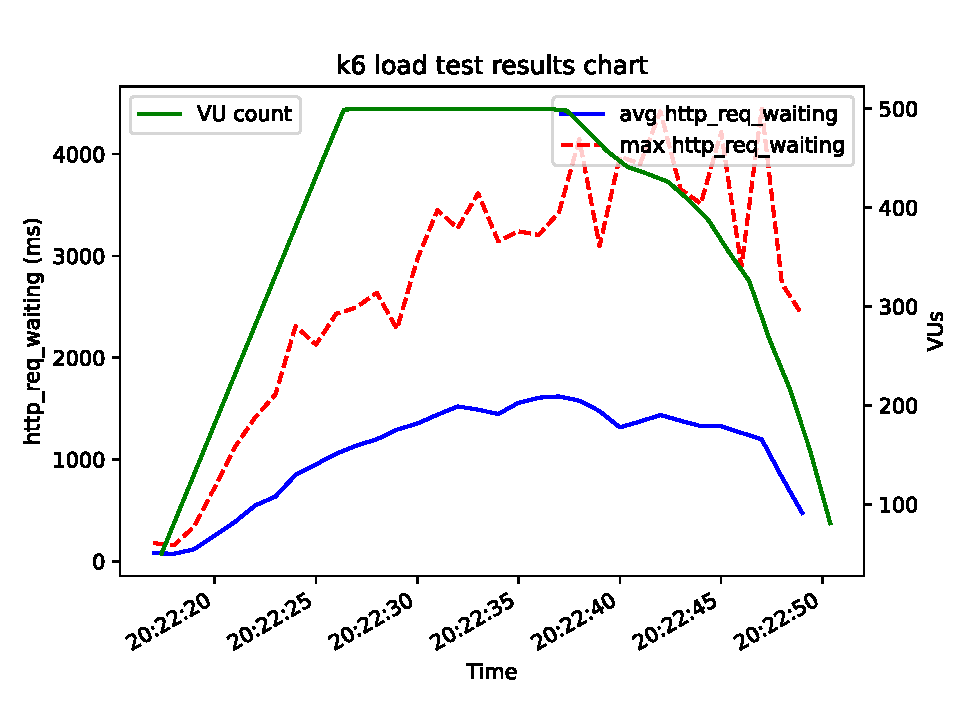
\includegraphics[width=1\textwidth]{pdf/visualizer-example.pdf}
    \caption{An example chart produced by the visualization script}
\end{figure}

Such visualization is possible because k6 tool supports exporting test results data to a JSON file by passing the argument \texttt{--out json=<file\_name>} to it.

Before the visualization can be done the JSON file containing test results has to be processed.
Each line of the file contains a JSON object containing either a metric definition or a measurement.
Developer can define custom metrics or use one of those that come predefined with the tool\footnote{\url{https://k6.io/docs/using-k6/metrics/#http-specific-built-in-metrics}}.

After all measurement objects have been parsed and processed a plot using the \texttt{matplotlib} library can be displayed.
The script also allows for exporting the created chart into a SVG file.

Due to the lack of free k6 test results visualization tools publicly available the author has decided to publish this script on GitHub \todo{repo link}.

\section{Results}
Dotypay Portal devices page takes 6+ seconds when there are more than 8000 terminals.

It should also be noted that after adding 7500 terminals to the application's database, the loading time of the table\footnote{A HTML table present in the GUI of the application, accessible after user authentication.} that displays available terminals has increased to an average of 6 seconds from previously measured 1 second in average.
The cause of this slowdown has not been identified yet and the team at Dotypay will further investigate it.

\end{document}
